\chapter{PENDAHULUAN}

\section{Latar Belakang}
Bisnis kuliner merupakan salah satu sektor usaha yang terus berkembang di Indonesia karena berkaitan langsung dengan kebutuhan konsumsi harian, perubahan gaya hidup masyarakat, serta meningkatnya pemanfaatan kanal digital dalam aktivitas pembelian makanan. Data Badan Pusat Statistik menunjukkan bahwa jumlah usaha penyediaan makanan dan minuman di Indonesia pada 2023 mencapai 4,85 juta usaha, meningkat 21,13\% dibandingkan 2016 yang berjumlah 4,01 juta usaha. Pada tahun yang sama, sektor ini menyerap 9,80 juta tenaga kerja dan menghasilkan nilai penjualan sebesar Rp998,37 triliun, meningkat 48,04\% dibandingkan 2016 \parencite{bps2024pmm}. Perkembangan tersebut berlanjut pada 2024, ketika jumlah usaha penyediaan makanan dan minuman di Indonesia meningkat menjadi 5,28 juta usaha \parencite{bps2025pmm}. Data ini menunjukkan bahwa usaha kuliner bukan hanya memiliki peran ekonomi yang besar, tetapi juga berkembang sebagai ruang usaha yang semakin padat pelaku.

Perkembangan usaha kuliner juga terlihat pada konteks Kota Medan. Sebagai pusat kegiatan ekonomi di Sumatera Utara, Kota Medan memiliki aktivitas konsumsi, perdagangan, dan jasa yang kuat. Dalam data PDRB menurut lapangan usaha, indikator BPS Kota Medan yang paling dekat dengan kegiatan kuliner berada pada kategori penyediaan akomodasi dan makan minum. Pada 2024, kategori ini menjadi lapangan usaha dengan pertumbuhan tertinggi di Kota Medan, yaitu 14,50\%, serta memiliki distribusi sebesar 3,06\% terhadap PDRB Kota Medan \parencite{bpsmedan2025ekonomi}. Kondisi tersebut memperlihatkan bahwa kegiatan makan dan minum menjadi bagian dari dinamika ekonomi perkotaan Medan yang terus bergerak, baik melalui usaha berskala besar maupun usaha kuliner lokal.

Tren perkembangan usaha kuliner nasional dan kategori penyediaan akomodasi dan makan minum di Kota Medan divisualisasikan pada Gambar~\ref{fig:tren-pdb-makan-minum-indonesia} dan Gambar~\ref{fig:tren-pdrb-makan-minum-medan}. Gambar~\ref{fig:tren-pdb-makan-minum-indonesia} menunjukkan bahwa PDB lapangan usaha penyediaan akomodasi dan makan minum atas dasar harga berlaku meningkat dari Rp394,06 triliun pada 2020 menjadi sekitar Rp638,41 triliun pada 2025. Sementara itu, Gambar~\ref{fig:tren-pdrb-makan-minum-medan} menunjukkan bahwa PDRB lapangan usaha penyediaan akomodasi dan makan minum di Kota Medan atas dasar harga berlaku meningkat dari Rp6,62 triliun pada 2020 menjadi Rp10,73 triliun pada 2025. Angka 2025 pada data Kota Medan merupakan angka sangat sementara dari BPS \parencite{bps2025pendapatan,bps2026ekonomiindonesia,bpsmedan2025pdrb,bpsmedan2026pdrb}. Dalam publikasi BPS, kategori ini mencakup penyediaan akomodasi jangka pendek serta penyediaan makanan dan minuman untuk konsumsi segera, sehingga digunakan sebagai indikator resmi yang paling dekat untuk membaca dinamika usaha kuliner dalam struktur PDRB Kota Medan \parencite{bpsmedan2025pdrb,bpsmedan2026pdrb}.

\begin{figure}[!t]
    \centering
    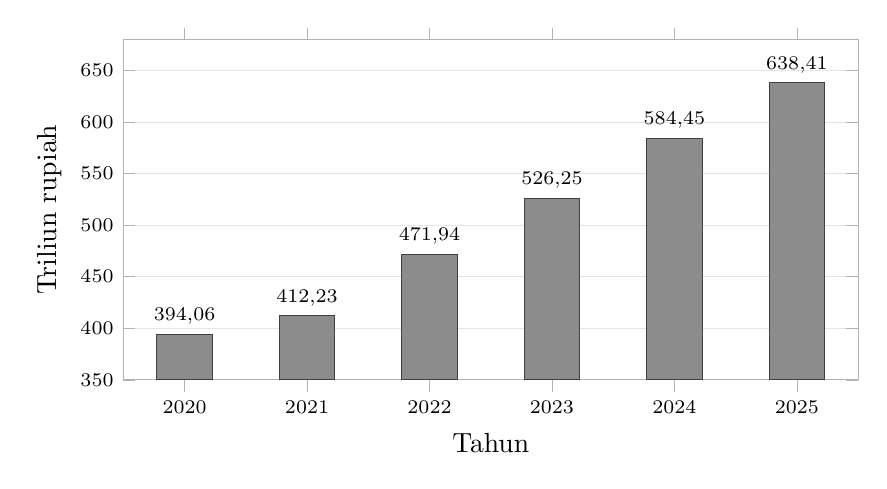
\begin{tikzpicture}
        \begin{axis}[
                width=0.9\textwidth,
                height=5.9cm,
                ybar,
                bar width=20pt,
                ymin=350, ymax=680,
                ylabel={Triliun rupiah},
                xlabel={Tahun},
                symbolic x coords={2020,2021,2022,2023,2024,2025},
                xtick=data,
                ymajorgrids=true,
                grid style={gray!20},
                axis line style={gray!60},
                tick style={gray!60},
                ytick={350,400,450,500,550,600,650},
                yticklabel style={font=\scriptsize},
                x tick label style={font=\scriptsize},
                enlarge x limits=0.10,
                clip=false
            ]
            \addplot[
                fill=black!45,
                draw=black!75
            ] coordinates {
                    (2020,394.06) (2021,412.23) (2022,471.94) (2023,526.25) (2024,584.45) (2025,638.41)
                };
            \node[font=\scriptsize, anchor=south] at (axis cs:2020,394.06) {394,06};
            \node[font=\scriptsize, anchor=south] at (axis cs:2021,412.23) {412,23};
            \node[font=\scriptsize, anchor=south] at (axis cs:2022,471.94) {471,94};
            \node[font=\scriptsize, anchor=south] at (axis cs:2023,526.25) {526,25};
            \node[font=\scriptsize, anchor=south] at (axis cs:2024,584.45) {584,45};
            \node[font=\scriptsize, anchor=south] at (axis cs:2025,638.41) {638,41};
        \end{axis}
    \end{tikzpicture}
    \figuresource[0.9\textwidth]{Diolah peneliti dari BPS \parencite{bps2025pendapatan,bps2026ekonomiindonesia}.}
    \caption{Tren PDB lapangan usaha penyediaan akomodasi dan makan minum di Indonesia atas dasar harga berlaku}
    \label{fig:tren-pdb-makan-minum-indonesia}
\end{figure}

\begin{figure}[!t]
    \centering
    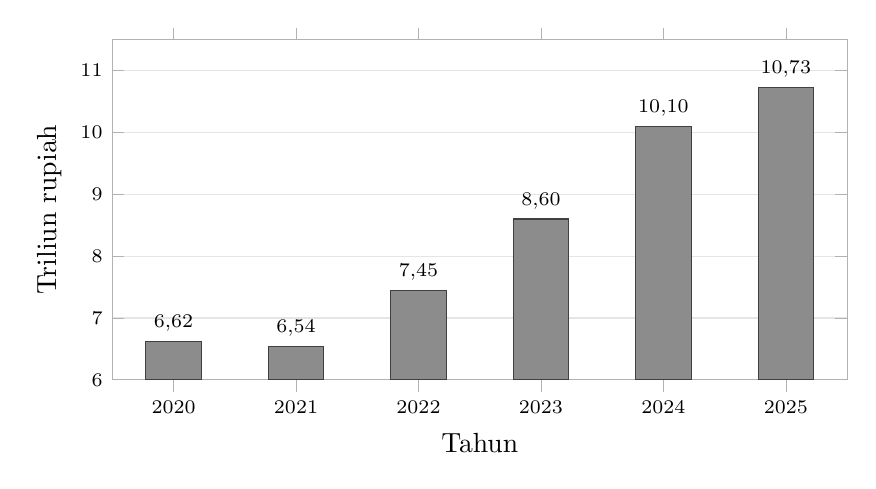
\begin{tikzpicture}
        \begin{axis}[
                width=0.9\textwidth,
                height=5.9cm,
                ybar,
                bar width=20pt,
                ymin=6, ymax=11.5,
                ylabel={Triliun rupiah},
                xlabel={Tahun},
                symbolic x coords={2020,2021,2022,2023,2024,2025},
                xtick=data,
                ymajorgrids=true,
                grid style={gray!20},
                axis line style={gray!60},
                tick style={gray!60},
                ytick={6,7,8,9,10,11},
                yticklabel style={font=\scriptsize},
                x tick label style={font=\scriptsize},
                enlarge x limits=0.10,
                clip=false
            ]
            \addplot[
                fill=black!45,
                draw=black!75
            ] coordinates {
                    (2020,6.62) (2021,6.54) (2022,7.45) (2023,8.60) (2024,10.10) (2025,10.73)
                };
            \node[font=\scriptsize, anchor=south] at (axis cs:2020,6.62) {6,62};
            \node[font=\scriptsize, anchor=south] at (axis cs:2021,6.54) {6,54};
            \node[font=\scriptsize, anchor=south] at (axis cs:2022,7.45) {7,45};
            \node[font=\scriptsize, anchor=south] at (axis cs:2023,8.60) {8,60};
            \node[font=\scriptsize, anchor=south] at (axis cs:2024,10.10) {10,10};
            \node[font=\scriptsize, anchor=south] at (axis cs:2025,10.73) {10,73};
        \end{axis}
    \end{tikzpicture}
    \figuresource[0.9\textwidth]{Diolah peneliti dari BPS Kota Medan \parencite{bpsmedan2025pdrb,bpsmedan2026pdrb}.}
    \caption{Tren PDRB lapangan usaha penyediaan akomodasi dan makan minum di Kota Medan atas dasar harga berlaku}
    \label{fig:tren-pdrb-makan-minum-medan}
\end{figure}

Pertumbuhan jumlah usaha kuliner menyebabkan tingkat persaingan semakin ketat. Pelaku usaha tidak hanya bersaing dari sisi rasa, tetapi juga dari variasi menu, harga, kemasan, lokasi, kecepatan layanan, promosi, reputasi, dan kemudahan akses pembelian. Dalam kondisi pasar yang padat, usaha kuliner membutuhkan strategi pemasaran yang efektif agar mampu menarik pelanggan baru, mempertahankan pelanggan lama, dan menjaga daya saing terhadap kompetitor. Pemasaran dalam konteks ini dipahami sebagai proses menciptakan, mengomunikasikan, menyampaikan, dan mempertukarkan nilai kepada konsumen \parencite{kotler2021marketingmanagement}. Oleh karena itu, strategi pemasaran perlu disusun berdasarkan pemahaman terhadap kebutuhan pasar, karakter konsumen, kekuatan usaha, serta tekanan persaingan yang dihadapi.

Pemasaran usaha kuliner dapat dilakukan melalui saluran offline dan online. Pemasaran offline umumnya dilakukan melalui lokasi fisik, papan nama, rekomendasi dari mulut ke mulut, pelayanan langsung, kerja sama komunitas, dan promosi di sekitar area usaha. Sementara itu, pemasaran online dilakukan melalui media sosial, katalog digital, mesin pencari, aplikasi pesan, marketplace, serta platform pesan antar makanan. Perkembangan pemasaran digital menjadi penting karena konsumen kini dapat menemukan, membandingkan, memesan, dan menilai produk kuliner melalui perangkat digital \parencite{chaffey2022digitalmarketing,regina2025kuliner}. Bagi UMKM kuliner, penggunaan kanal digital dapat memperluas jangkauan pasar, meningkatkan visibilitas, dan mempercepat transaksi ketika dikelola secara konsisten \parencite{regina2025kuliner,mamuriyah2021gadihminang,roslam2021markisaaurora,suharjo2020bogorsnacks}.

Salah satu bentuk pemasaran online yang banyak digunakan pelaku usaha kuliner adalah platform marketplace atau \textit{online food delivery} seperti ShopeeFood, GoFood, dan GrabFood. Platform tersebut tidak hanya berfungsi sebagai media pemesanan, tetapi juga menjadi etalase digital yang menampilkan nama usaha, foto menu, harga, promo, rating, ulasan pelanggan, dan estimasi layanan. Kajian terdahulu menunjukkan bahwa pemanfaatan platform digital dapat membantu UMKM memperluas jangkauan pasar dan meningkatkan penjualan ketika fitur platform, promosi, tampilan produk, serta komunikasi dengan pelanggan dikelola secara konsisten \parencite{regina2025kuliner,sophia2025rendanggadih,suharjo2020bogorsnacks}. Hal ini menunjukkan bahwa platform seperti GrabFood telah menjadi ruang pemasaran dan persaingan yang penting bagi usaha kuliner.

Rumah Makan Nasi Gerilya merupakan usaha nasi Padang di Kota Medan yang memanfaatkan kanal online dalam aktivitas penjualannya. Berdasarkan wawancara awal dengan pemilik, Nasi Gerilya menggunakan GrabFood, GoFood, dan ShopeeFood sebagai kanal penjualan online, tetapi GrabFood menjadi platform utama karena dinilai paling sesuai dengan target pasar usaha. Pemilik juga menyampaikan bahwa GrabFood berkontribusi lebih dari 50\% terhadap \textit{revenue} usaha, sehingga platform ini tidak hanya berperan sebagai saluran tambahan, tetapi sebagai salah satu kanal penjualan utama. Hasil observasi toko pada GrabFood menunjukkan bahwa Nasi Gerilya memiliki rating 4,7/5,0, 4.187 ulasan, rentang harga Rp11.000--Rp72.000, promo platform aktif, serta menu teratas seperti rendang sapi, ayam goreng, ayam bakar, dan nasi bakar kikil tunjang. Keempat menu teratas tersebut menunjukkan variasi harga utama yang ditawarkan Nasi Gerilya pada GrabFood sebagaimana disajikan pada Tabel~\ref{tab:harga-menu-teratas-gerilya}.

\begin{table}[!t]
    \centering
    \caption{Harga Menu Teratas Rumah Makan Nasi Gerilya pada GrabFood}
    \label{tab:harga-menu-teratas-gerilya}
    \small
    \renewcommand{\arraystretch}{1.08}
    \begin{tabularx}{0.82\textwidth}{|X|>{\raggedleft\arraybackslash}p{3cm}|}
        \toprule
        \textbf{Menu Teratas}    & \textbf{Harga} \\ \hline
        \midrule
        Nasi Padang Rendang Sapi & Rp56.000       \\ \hline
        Nasi Padang Ayam Goreng  & Rp45.000       \\ \hline
        Nasi Padang Ayam Bakar   & Rp45.000       \\ \hline
        Nasi Bakar Kikil Tunjang & Rp68.000       \\ \hline
        \bottomrule
    \end{tabularx}
    \tablesource[0.82\textwidth]{Observasi platform GrabFood pada 04 April 2026; diolah peneliti (2026).}
\end{table}

Menu selebihnya disajikan secara lebih lengkap pada Lampiran Tabel~\ref{tab:survei_harga_nasi_gerilya_grabfood}. Data awal mengenai observasi GrabFood, wawancara awal pemilik, dan dokumentasi kinerja usaha disajikan lebih lengkap pada Lampiran~\ref{app:observasi-grabfood}, Lampiran~\ref{app:wawancara-awal-pemilik}, dan Lampiran~\ref{app:dokumentasi-indeks-kinerja}. Visual pendukung pada Gambar~\ref{fig:tren-penjualan-bungkus-gerilya} menunjukkan bahwa jumlah penjualan Nasi Gerilya meningkat dari 6.702 bungkus pada Desember 2024 menjadi 16.590 bungkus pada Maret 2025, tetapi kemudian menurun bertahap menjadi 12.900 bungkus pada November 2025. Gambar~\ref{fig:komposisi-pelanggan-gerilya} juga menunjukkan bahwa pelanggan baru meningkat dari 45\% menjadi 55\%, sedangkan \textit{repeat order} menurun dari 43\% menjadi 38\%. Kondisi tersebut menunjukkan bahwa eksposur digital dan kontribusi GrabFood yang besar belum otomatis menjamin stabilitas penjualan dan loyalitas pelanggan.

\begin{figure}[!t]
    \centering
    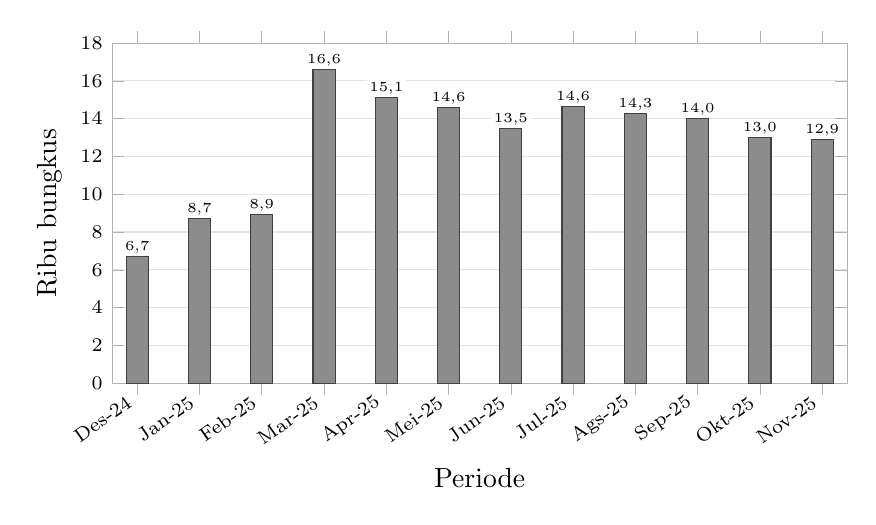
\begin{tikzpicture}
        \begin{axis}[
                width=0.9\textwidth,
                height=5.9cm,
                ybar,
                bar width=8pt,
                xmin=-0.4, xmax=11.4,
                ymin=0, ymax=18,
                ylabel={Ribu bungkus},
                xlabel={Periode},
                ymajorgrids=true,
                grid style={gray!20},
                axis line style={gray!60},
                tick style={gray!60},
                xtick=data,
                xticklabels={Des-24,Jan-25,Feb-25,Mar-25,Apr-25,Mei-25,Jun-25,Jul-25,Ags-25,Sep-25,Okt-25,Nov-25},
                x tick label style={rotate=35, anchor=east, font=\scriptsize},
                ytick={0,2,4,6,8,10,12,14,16,18},
                yticklabel style={font=\scriptsize},
                clip=false
            ]
            \addplot[
                fill=black!45,
                draw=black!75
            ] coordinates {
                    (0,6.702) (1,8.740) (2,8.911) (3,16.590) (4,15.129) (5,14.580)
                    (6,13.467) (7,14.633) (8,14.259) (9,14.034) (10,13.009) (11,12.900)
                };
            \node[font=\tiny, fill=white, inner sep=1pt, anchor=south] at (axis cs:0,6.702) {6,7};
            \node[font=\tiny, fill=white, inner sep=1pt, anchor=south] at (axis cs:1,8.740) {8,7};
            \node[font=\tiny, fill=white, inner sep=1pt, anchor=south] at (axis cs:2,8.911) {8,9};
            \node[font=\tiny, fill=white, inner sep=1pt, anchor=south] at (axis cs:3,16.590) {16,6};
            \node[font=\tiny, fill=white, inner sep=1pt, anchor=south] at (axis cs:4,15.129) {15,1};
            \node[font=\tiny, fill=white, inner sep=1pt, anchor=south] at (axis cs:5,14.580) {14,6};
            \node[font=\tiny, fill=white, inner sep=1pt, anchor=south] at (axis cs:6,13.467) {13,5};
            \node[font=\tiny, fill=white, inner sep=1pt, anchor=south] at (axis cs:7,14.633) {14,6};
            \node[font=\tiny, fill=white, inner sep=1pt, anchor=south] at (axis cs:8,14.259) {14,3};
            \node[font=\tiny, fill=white, inner sep=1pt, anchor=south] at (axis cs:9,14.034) {14,0};
            \node[font=\tiny, fill=white, inner sep=1pt, anchor=south] at (axis cs:10,13.009) {13,0};
            \node[font=\tiny, fill=white, inner sep=1pt, anchor=south] at (axis cs:11,12.900) {12,9};
        \end{axis}
    \end{tikzpicture}
    \figuresource[0.9\textwidth]{Diolah peneliti dari dokumentasi grafik penjualan bulanan Nasi Gerilya.}
    \caption{Tren jumlah penjualan bulanan Nasi Gerilya dalam satuan bungkus}
    \label{fig:tren-penjualan-bungkus-gerilya}
\end{figure}

\begin{figure}[!t]
    \centering
    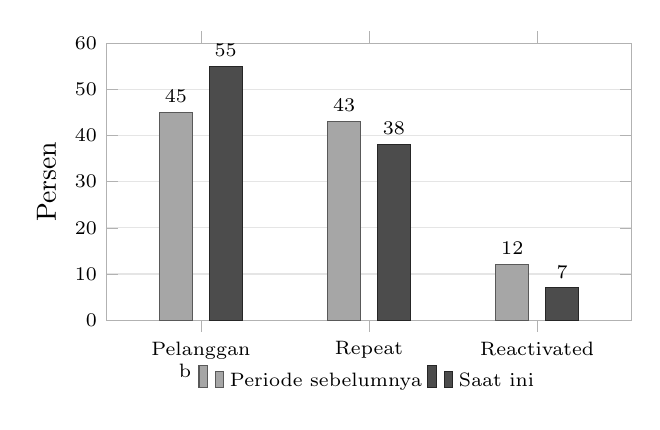
\begin{tikzpicture}
        \begin{axis}[
                width=0.68\textwidth,
                height=5.1cm,
                ybar=6pt,
                bar width=12pt,
                ymin=0, ymax=60,
                ylabel={Persen},
                ymajorgrids=true,
                grid style={gray!20},
                axis line style={gray!60},
                tick style={gray!60},
                symbolic x coords={Baru,Repeat,Reactivated},
                xtick=data,
                xticklabels={Pelanggan\\baru,Repeat\\order,Reactivated},
                x tick label style={font=\scriptsize, align=center},
                ytick={0,10,20,30,40,50,60},
                yticklabel style={font=\scriptsize},
                nodes near coords,
                every node near coord/.append style={font=\scriptsize},
                enlarge x limits=0.28,
                legend style={
                        font=\scriptsize,
                        draw=none,
                        at={(0.5,-0.14)},
                        anchor=north,
                        legend columns=2
                    }
            ]
            \addplot[fill=black!35, draw=black!65] coordinates {(Baru,45) (Repeat,43) (Reactivated,12)};
            \addplot[fill=black!70, draw=black!85] coordinates {(Baru,55) (Repeat,38) (Reactivated,7)};
            \legend{Periode sebelumnya,Saat ini}
        \end{axis}
    \end{tikzpicture}
    \figuresource[0.68\textwidth]{Diolah peneliti dari wawancara awal dengan pemilik usaha.}
    \caption{Perubahan komposisi pelanggan Nasi Gerilya berdasarkan wawancara awal pemilik usaha}
    \label{fig:komposisi-pelanggan-gerilya}
\end{figure}
Dalam kondisi tersebut, bauran pemasaran atau \textit{marketing mix} menjadi konsep yang relevan untuk membaca strategi pemasaran Nasi Gerilya. Konsep 4P menempatkan \textit{product}, \textit{price}, \textit{place}, dan \textit{promotion} sebagai perangkat utama dalam mengelola penawaran pasar \parencite{kotler2023principlesmarketing}. Pada bisnis jasa dan kuliner, bauran tersebut dapat diperluas menjadi 7P dengan menambahkan \textit{people}, \textit{process}, dan \textit{physical evidence} karena pengalaman pelanggan juga dipengaruhi oleh pelaksana layanan, proses pemenuhan pesanan, serta bukti kualitas yang terlihat oleh konsumen \parencite{wirtz2024servicesmarketing}. Dalam konteks Nasi Gerilya pada GrabFood, unsur produk terlihat dari variasi menu dan konsistensi rasa; harga terlihat dari rentang harga, ongkos kirim, dan promo; tempat terlihat dari penggunaan GrabFood sebagai kanal distribusi online; promosi terlihat dari voucher, promo platform, media sosial, dan KOL; \textit{people} terlihat dari kesiapan admin, karyawan, dan juru masak; \textit{process} terlihat dari kecepatan layanan, pengelolaan menu habis, dan ketepatan pesanan; sedangkan \textit{physical evidence} terlihat dari foto produk, kemasan, rating, dan ulasan pelanggan.

Review pelanggan menjadi bagian penting dalam evaluasi strategi pemasaran karena platform \textit{online food delivery} membuat pengalaman pelanggan terekam secara terbuka melalui rating, komentar, keluhan, dan rekomendasi. Penelitian terdahulu menunjukkan bahwa harga, promosi, tampilan produk, kualitas layanan, ulasan, dan peringkat pada platform digital dapat memengaruhi keputusan pembelian serta performa penjualan usaha kuliner \parencite{sophia2025rendanggadih,ruhiyat2023minatbeli,khairani2022buahsayur,suharjo2020bogorsnacks}. Pada Nasi Gerilya, review pelanggan memuat komentar positif mengenai rasa enak, bumbu dan rempah yang kuat, porsi besar, bahan segar, kemasan rapi, variasi menu, serta harga yang dinilai terjangkau. Namun, review tersebut juga memuat keluhan mengenai rasa yang dianggap berubah, pesanan tidak lengkap, menu tidak tersedia, lauk utama yang dinilai kurang besar atau kurang segar, nasi yang kadang keras, proporsi nasi dan lauk yang kurang seimbang, serta suhu makanan yang tidak selalu konsisten. Oleh karena itu, review pelanggan, komentar, keluhan, dan permasalahan layanan menjadi dasar penting untuk mengevaluasi serta meningkatkan strategi pemasaran Nasi Gerilya pada GrabFood.

\section{Rumusan Masalah}
Berdasarkan latar belakang di atas, maka rumusan masalah dalam penelitian ini adalah:
\begin{enumerate}
    \item Bagaimana faktor internal Rumah Makan Nasi Gerilya pada platform GrabFood yang mencakup kekuatan dan kelemahan usaha?
    \item Bagaimana faktor eksternal Rumah Makan Nasi Gerilya pada platform GrabFood yang mencakup peluang dan ancaman usaha?
    \item Bagaimana strategi pemasaran Rumah Makan Nasi Gerilya pada platform GrabFood berdasarkan analisis matriks SWOT?
\end{enumerate}

\section{Tujuan Penelitian}
Tujuan yang ingin dicapai dalam penelitian ini adalah sebagai berikut:
\begin{enumerate}
    \item Untuk mengidentifikasi faktor internal Rumah Makan Nasi Gerilya pada platform GrabFood yang mencakup kekuatan dan kelemahan usaha.
    \item Untuk mengidentifikasi faktor eksternal Rumah Makan Nasi Gerilya pada platform GrabFood yang mencakup peluang dan ancaman usaha.
    \item Untuk merumuskan strategi pemasaran Rumah Makan Nasi Gerilya pada platform GrabFood berdasarkan analisis matriks SWOT.
\end{enumerate}

\section{Manfaat Penelitian}
Penelitian ini diharapkan dapat bermanfaat secara teoretis dan praktis:
\subsection{Manfaat Teoretis}
Penelitian ini diharapkan dapat berkontribusi dalam pengembangan ilmu manajemen pemasaran, khususnya yang berkaitan dengan strategi pemasaran usaha kuliner pada platform \textit{online food delivery}, terutama GrabFood. Selain itu, penelitian ini juga diharapkan dapat memperkaya kajian mengenai penerapan analisis SWOT dalam mengidentifikasi faktor internal dan faktor eksternal usaha sebagai dasar perumusan strategi pemasaran. Hasil penelitian ini selanjutnya diharapkan dapat menjadi bahan referensi bagi peneliti lain yang ingin mengkaji topik serupa, terutama pada konteks UMKM kuliner yang memanfaatkan platform digital sebagai saluran pemasaran.
\subsection{Manfaat Praktis}
Secara praktis, penelitian ini diharapkan dapat memberikan manfaat bagi beberapa pihak sebagai berikut:
\subsubsection{Bagi Rumah Makan Nasi Gerilya}
\noindent Penelitian ini diharapkan dapat menjadi bahan masukan dan evaluasi dalam mengidentifikasi kekuatan, kelemahan, peluang, dan ancaman usaha pada platform GrabFood. Dengan demikian, hasil penelitian ini dapat digunakan sebagai dasar dalam merumuskan strategi pemasaran yang lebih tepat untuk mempertahankan daya saing dan meningkatkan kinerja usaha.
\subsubsection{Bagi Pelaku Usaha Kuliner}
\noindent Penelitian ini diharapkan dapat menjadi gambaran dan bahan pertimbangan bagi pelaku usaha kuliner lainnya mengenai pentingnya analisis kondisi internal dan eksternal usaha dalam menyusun strategi pemasaran pada platform \textit{online food delivery}.
\subsubsection{Bagi Akademisi}
\noindent Penelitian ini diharapkan dapat menjadi tambahan acuan dan referensi ilmiah, khususnya yang berkaitan dengan strategi pemasaran kuliner berbasis platform, strategi pemasaran UMKM, dan penerapan analisis SWOT pada sektor kuliner.
